\title{Physics 134 
\partition\
\vspace{1ex}
Measurement of the Lifetime of a Muon\\
\vspace{1ex}
\normalsize{ Rick Ramirez}}
\date{Spring 2016}
\documentclass[12pt]{article}
\usepackage[margin=0.8in]{geometry}
\usepackage{amsmath, amssymb, enumerate} %amssymb provides symbols for (integers, reals etc.)
\usepackage{verbatim} % Comment block.
\usepackage{pgfplots} % 3D plots
\pgfplotsset{compat=1.8}
\usepackage{mathrsfs} % provides cursive letters
\usepackage{caption}
\usepackage{booktabs,color,soul}
\linespread{1.3}
\newcommand{\partition}{\rule{\linewidth}{0.8pt}}
\soulregister\cite7
\soulregister\ref7
% my own titles
\makeatletter
\renewcommand{\maketitle}{
\begin{center}
\@date \hfill  \@author\\
{\Large \textsc{\@title}}
\partition\\
\end{center}
}
\usepackage{tikz}
\DeclareRobustCommand{\hlcyan}[1]{{\sethlcolor{cyan}\hl{#1}}}
\newcommand{\highlight}[1]{%
  \colorbox{yellow!100}{$\displaystyle#1$}}

%%%----------%%%----------%%%----------%%%----------%%%----------%%%
%%%----------%%%----------%%%----------%%%----------%%%----------%%%

\begin{document}
\maketitle
\linespread{1.5}
\abstract{By measuring light pulses produced by incoming particles through a plastic scintillator, we aimed to measure the lifetime of a muon. The device was allowed to run for $94$ hours and recorded $7558$ events. Analysis of the data produced a lifetime of $2.017 \pm 0.02 \mu s$}, which was used to calculate a Fermi coupling constant value of $1.205 \pm 0.006 \times 10^{-5}GeV^{-2}$.
\section{Introduction}
\noindent
As cosmic rays strike the top of Earth's atmosphere, they interact with the nuclei of air molecules. This produces a range of particles, particularly pions. A pion that does not interact with the nuclei of surrounding molecules will decay via weak interactions. The outcome of this type of interaction produces both muons and neutrinos
\begin{equation}
\begin{split}
  & \pi^+ \longrightarrow \mu^+ \nu_{\mu}
  \\
  & \pi^- \longrightarrow \mu^- \bar{\nu}_{\mu}
  \end{split}
  \end{equation}  
The muons that are produced travel toward the surface of earth at near the speed of light, however, because a muon may interact with matter via weak and electromagnetic forces, it looses kinetic energy along its trajectory.  Most muons are produced at an altitude of approximately $15$ km, and if traveling at the speed of light, require a transit time of $50\mu$s. The average lifetime of a muon at rest is approximately $2\mu$s, but due to relativistic effects, there is an average flux of $1$ muon min$^{-1}$cm$^{-2}$ at sea-level \cite{Beatty}. 

The mean energy of muons that reach sea-level is about $4$GeV and the energy loss through coulombic interactions through matter is about $2$MeV g$^-1$ cm$^{2}$. Because the interaction length of the atmosphere is about $1000$ g cm$^{-2}$, the original energy of a muon detected at sea-level is roughly $6$ GeV. Given the dimensions of the scintillator from Table \ref{tab:scintillator}, the muons that manage to stop and decay in the detector have a total energy of about $160$ MeV as they enter the cylinder. 

\section{Experimental Setup}
The detector is composed of a plastic sciltillator that is monitored by a photomultiplier tube which is in turn connected to an adjustable high voltage and a discriminator, followed by an FPGA timer, and finally a computer as shown in Fig.\ref{fig:electronics}. As a particle enters the cylinder, scintillation light is produced and detected by the photomultiplier tube.  The signal output signal feeds a two stage amplifier that feeds the discriminator. For signals above the threshold, a transistor-transistor logic output pulse is produced, which triggers the timing circuit of the FPGA. A second signal arriving at the FPGA within a fixed time interval resets the timing circuit, and the event is recorded. 

\begin{figure}[h]
\begin{center}
 \quad 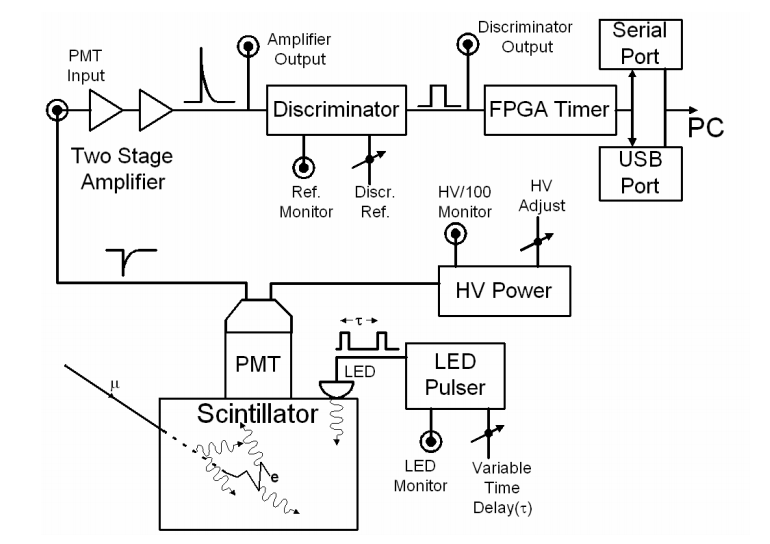
\includegraphics[width=0.6\textwidth]{electronics}
\end{center}
\caption{Block diagram of electronics. Taken from \cite{manual}.}
\label{fig:electronics}
\end{figure}
\begin{table}[htbp]\centering
\begin{tabular}{ |p{3cm}|p{3cm}|}
 \hline
  Mass density & \qquad $1.032 \frac{\text{g}}{\text{cm}^3}$\\
 \hline
Refractive index & \qquad $1.58$\\
\hline
 Diameter & \qquad $15$ cm\\
 \hline
 Height & \qquad $12.5$ cm\\
 \hline
\end{tabular}
\def\sym#1{\ifmmode^{#1}\else\(^{#1}\)\fi}
\caption{Scintillator dimensions and properties. Adapted from \cite{manual}}
\label{tab:scintillator}
\end{table}

\section{Procedure}
The threshold of the detector controls the voltage output. Sine waves sent from a function generator to the discriminator produce a square pulse output. The timing properties of the FPGA can be verified by using the pulser located in the detector. Figure 2 show a plot of the time between successive pulses as measured by an oscilloscope and the FPGA. Altering the time between rising edges of detector pulser demonstrates the linearity of the FPGA.  



\begin{figure}[h]
\begin{center}
 \quad 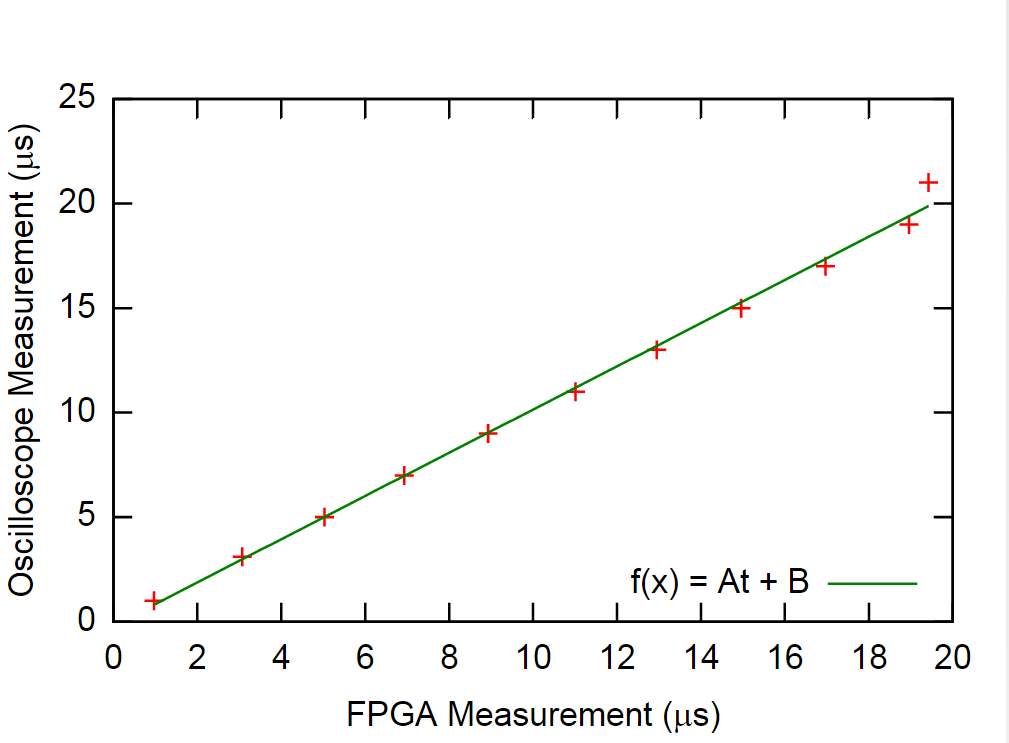
\includegraphics[width=0.6\textwidth]{FPGA_linearity}
\end{center}
\caption{ Measurements of the time between successive rising edges. The x-axis corresponds to measurements made by the FPGA and the y-axis corresponds to an oscilloscope. The slope between the two is approximately 1.}
\label{fig:linear}
\end{figure}

Figure \ref{fig:linear} shows shat the maximum time between successive pulses registered is around $20\mu$s, which implies that increasing the number of bins above this value should have no effect on the spread of the data. This is the result of the timing circuit being reset, during which the FPGA no longer records results. A linear fit of the data produces a slope of $1.03 \pm 0.02 \mu$s. The result of decreasing the time interval between successive pulses indicates that the minimum internal timing bin width is about $0.02\mu$s. This value corresponds to the resolution of the FPGA.  In terms of events, increasing the threshold of the discriminator correlates to an decrease in the number of pulses with decay fluctuations ranging from $20n$s to $1180n$s. With the information at hand, we set the discriminator to a final value of $220$mV, and proceeded to examine the high voltage. By monitoring the muon count rate, we increased the voltage and attempted to determine then end of the plateau region. Figure \ref{fig:HV} shows a sharp increase between $1050$ and $1100$V. A value of $1100$V was used for the remainder of the experiment.
\begin{figure}[h]
\begin{center}
 \quad 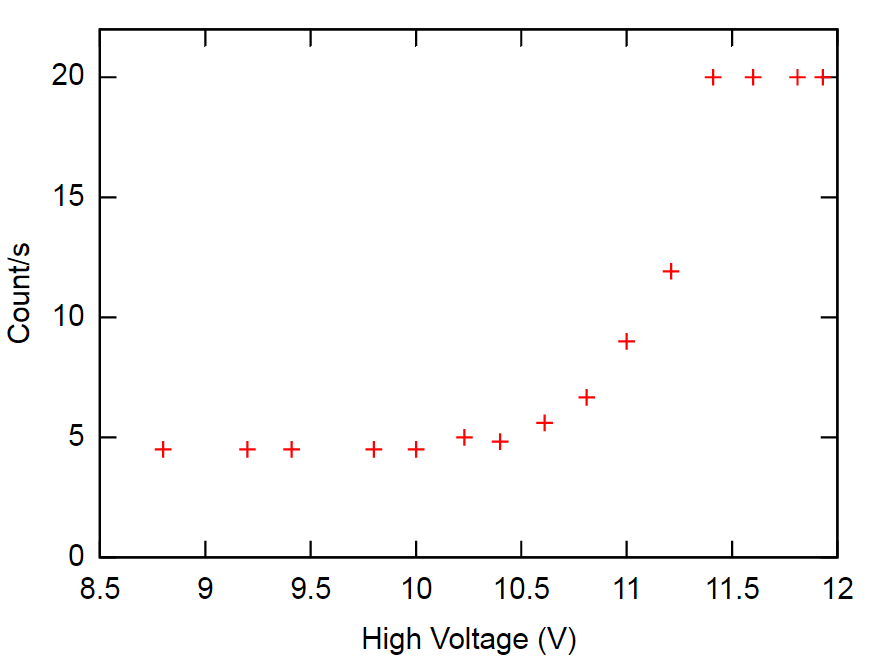
\includegraphics[width=0.7\textwidth]{gnuHV}
\end{center}
\caption{Muon count rate as a function of Voltage.}
\label{fig:HV}
\end{figure}

\section{Analysis}
The detector was allowed to run for a total of $94$ hours during which time, $3091355$ events were recorded. Timing data greater than $40000$ns indicates a scenario where the time between successive signals exceeded the maximum number of clock cycles. After sifting the data, we were left with total $7558$ events. As shown in Fig. \ref{fig:lifetime}, the data were arranged into bins of width $0.1\mu$s for  events with pulse separations between $0$ and $10\mu$s which produced $99$ bins. Our next task was to fit an exponentially decaying function to the data.  With the number of events in bin $j$ denoted by $d_j$, with statistical variance $\sqrt{d_j}$ and a fitting function of
\begin{equation}
y(t_j) = A\:\exp (-t_j/\tau) + B\:,
\end{equation}
our goal is to find values of $A$, $B$, and $\tau$ that minimized the sum of the squares of the normalized discrepancies $\chi^2$ defined as
\begin{equation}
\chi^2 \equiv \sum_{j=1}^N\frac{(y_j - d_j)^2}{\sigma^2} = \sum_{j=1}^N\frac{(y_j - d_j)^2}{d_j}\:.
\end{equation}
Inserting the trial function in Eq.2, and minimizing with respect to $A$ and $B$ produces
\begin{equation}
\begin{split}
\frac{\partial \chi^2}{\partial A} & = \sum \left[ \frac{2}{d_j}[(A\exp (-t_j/\tau) + B)\exp(-t_j/\tau)] -2\exp(-t_j/\tau) \right] = 0
\\
& \qquad\qquad\qquad\qquad\qquad\text{and}
\\
\frac{\partial \chi^2}{\partial B} & = \sum\left[ \frac{2}{d_j}[A\exp(-t_j/\tau) + B] - 2 \right] = 0
\end{split}
\end{equation}
While holding $\tau$ constant at a value of $2\mu$s, we are free to minimize the two equations. This is achieved by evaluating the following sums
\begin{equation}
\begin{split}
& N \equiv \sum 1 \qquad \alpha \equiv \sum d_j \qquad \beta \equiv \sum \exp(t_j/\tau)
\\[2ex]
& \gamma \equiv \sum\frac{1}{d_j} \qquad \delta \equiv \sum\frac{\exp(t_j/\tau)}{d_j} \qquad \lambda \equiv \frac{\exp(-2t_j/\tau)}{d_j}\:,
\end{split}
\end{equation}
and is summarized in table 2.

\begin{table}[htbp]\centering
\begin{tabular}{ |p{0.5cm}|p{3cm}|}
 \hline
  N & \qquad $99$\\
 \hline
$\alpha$ & \qquad $7119$\\
\hline
 $\beta$ & \qquad $19.04$ \\
 \hline
 $\gamma$ & \qquad $5.61$ \\
 \hline
 $\delta$ & \qquad $0.23$ \\
 \hline
 $\lambda$ & \qquad $0.055$ \\
 \hline
\end{tabular}
\def\sym#1{\ifmmode^{#1}\else\(^{#1}\)\fi}
\caption{Numerical evaluation of sums in Eq.5}
\end{table}
\noindent
Inserting the variables from Eqn.5 into Eqn.4, we can solve for $A$ and $B$.
\begin{equation}
\begin{split}
A = \frac{\beta\gamma - N\delta}{\lambda\gamma - \delta^2} = 361.74 \qquad\text{and}\qquad B = \frac{N\lambda - \beta\delta}{\lambda\gamma - \delta^2} = 2.86
\end{split}\:.
\end{equation}
Re-writing the equation for $\chi^2$ in terms of the variables in Eqn.5, we obtain
\begin{equation}
\chi^2 = \lambda A^2 + 2\delta AB + \gamma B^2 - 2\beta A - 2NB + \alpha = 86.04
\end{equation}

Holding $A$ and $B$ as they are in Eqn.6, it was found that the lowest value obtainable is $\chi^2 = 85.26$, corresponding to a lifetime value of $2.017\mu$s. Varying $\tau$ by hand and allowing A and B to vary as well, produces a value of $\chi^2 = 82.31$ and a life time of $\tau = 2130\mu s$\\

With $3$ free parameters and $N = 99$ bins, we are left with $\nu = 96$ degrees of freedom. For an appropriate fitting function, the goodness of fit should fall between 
\begin{equation}
\begin{split}
\nu - \sqrt{2\nu} \leq & \chi^2\leq\nu + \sqrt{2\nu} \quad\text{for}\quad\nu\geq 30
\\
82.14 \leq & \chi^2 \leq 109.86
\end{split}
\end{equation}
With the value of $\chi^2 = 82.31$, we are free to calculate the variance of the parameters.  An estimation on the variance of the three parameters was obtained by holding two variables static, and varying the third until the goodness of fit increased a factor of $1+\sqrt{2/\nu} = 1.144$. The optimal values of the three parameters, along with their calculated variances, are summarized in Table 3, and a plot of the data can be found in Fig.4.
\begin{table}[htbp]\centering
\begin{tabular}{ |p{0.5cm}|p{4cm}|}
 \hline
$A$ & \qquad $347.731 \pm 4.77$\\
\hline
 $B$ & \qquad $1.225 \pm 0.26$ \\
 \hline
 $\tau$ & \qquad $2.125 \pm 0.02\:\mu s$\\
 \hline
\end{tabular}
\def\sym#1{\ifmmode^{#1}\else\(^{#1}\)\fi}
\caption{Calculation of the values for parameters of fitting function. }
\end{table}
\begin{figure}[h]
\begin{center}
 \quad 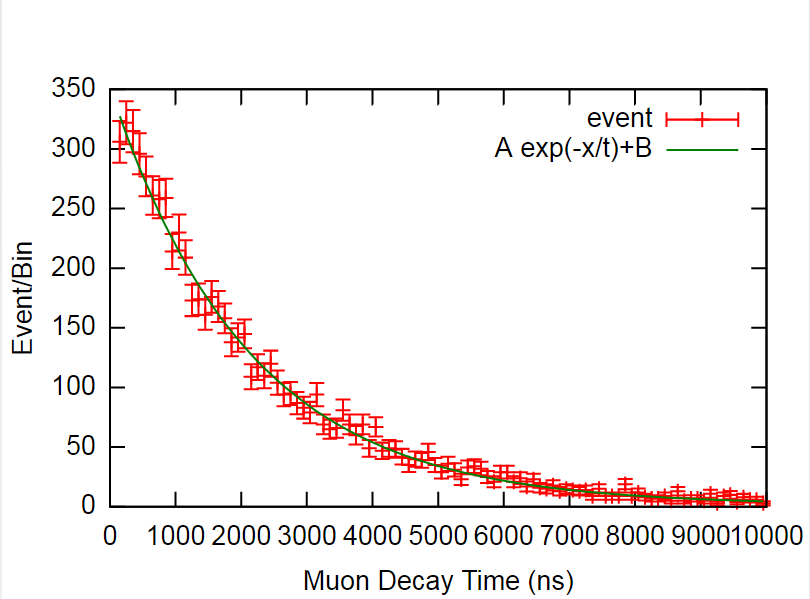
\includegraphics[width=0.9\textwidth]{gnuMuonPlot}
\end{center}
\caption{Decay time for 7558 events collected over 94 hours. The error on each point is $\sqrt{d_j}$, where $d_j$ is the number of events in bin $j$.}
\label{fig:lifetime}
\end{figure}

\noindent
To get a more precise fit to the data, a least square approach was also used. The data was binned the same as above and fit to the decaying exponential
\begin{equation}
N(t) = Ae^{-\frac{t}{\tau_{\mu}}} + B\:,
\end{equation} 
where $\tau_{\mu}$ is the mean muon lifetime, $A$ is a normalization constant, and B is number of background events per time bin. The values of the initial parameters were set to the values calculated above. All three parameters were allowed to vary until a convergence was reached. The results of this method can be seen in Table \ref{tab:gnutab}, and a plot can be seen in Fig. \ref{fig:lifetime}. For 96 degrees of freedom and a $\chi^2$ value of 76.64, the confidence level is \%93.81.
\begin{table}[h!]\centering
\begin{tabular}{ |p{0.5cm}|p{4cm}|}
 \hline
$A$ & \qquad $350.005 \pm 6.155$\\
\hline
 $B$ & \qquad $1.471 \pm 0.692$ \\
 \hline
 $\tau$ & \qquad $2.109 \pm 0.04\:\mu s$\\
 \hline
 $\chi^2$ & \qquad $75.64$\\
 \hline
\end{tabular}
\def\sym#1{\ifmmode^{#1}\else\(^{#1}\)\fi}
\caption{Values for parameters of fitting function produced by gnuplot.}
\label{tab:gnutab}
\end{table}

\newpage
With the value of the muon lifetime measured, we can now calculate the value and corresponding error of the Fermi coupling constant  
\begin{equation}
\frac{G_f}{(\hbar c)^3} = \sqrt{\frac{192\pi^3\hbar}{\tau m^5}}\:.
\end{equation}
The current value measured values of the mass of a muon at rest and Planck's constant are $m_{\mu} = 105.65837(35)$MeV and $\hbar = 6.58211899(16)\times 10^{-22}$ MeV s. Compared to the level of uncertainty in the measurement of the muon lifetime above, these values can be taken to be constant to three significant digits. The speed of light in a vacuum is $c = 299792458 \text{ m s}^{-1}$ and is taken to be exact. \cite{pdg, pdg2, nist}.

\begin{equation}
\frac{G_f}{(\hbar c)^3} = \sqrt{\frac{192\pi^3(6.582\times 10^{-25}GeV\cdot s)}{(2.109\times 10^{-6}s)(0.106\:GeV)^5}} = 1.178 \times 10^{-5}\: GeV^{-2} 
\end{equation}

\begin{equation}
\sigma_G^2  = \left( \frac{\partial G}{\partial \tau} \right)^2\sigma_{\tau}^2 =   \left[- \frac{1}{2}\left( \frac{1}{\tau} \right)^{3/2}\sqrt{\frac{192\pi^3\hbar}{ m^5}}\right]^2\:\sigma_{\tau}^2  
\end{equation}

\begin{equation}
\frac{G_f}{(\hbar c)^3} = 1.178 \pm 0.0119 \times 10^{-5}GeV^{-2}
\end{equation}
The value of the coupling constant reported by the Particle Data Group is \cite{pdg2}
\begin{equation}
\frac{G_f}{(\hbar c)^3} = 1.166 37(1)\times 10^{-5}GeV^{-2}\:.
\end{equation}
The calculated value of $\tau = 2.109\pm 0.004\mu$s being less than that of the lifetime of a muon in free space, $\tau_{free} = 2.19698(22)\mu$s is reasonable due to the fact that the incoming muons can have positive or negative charge. Unlike the positive muon, a negative particle that stops inside the scintillator will tend to bind to the carbon and hydrogen nuclei with the effect of producing a shorter measured lifetime.
\section{Conclusion}
By measuring pulses of scintillation light produced by incoming particles, we were able to measure a muon lifetime of $\tau = 2.109\pm 0.004\:\mu$s. The observed value was  lower than the lifetime of a muon in free space ($\tau_{free} = 2.19698(22)\:\mu$s) as expected. With this measurement, we were able to calculate the value of the Fermi coupling constant $G_f /(\hbar c)^3 = 1.178 \pm 0.0119 \times 10^{-5}GeV^{-2}$, which agrees with the value $1.166 37(1)\times 10^{-5}GeV^{-2}$ to within three decimal places of error.







\newpage
\begin{thebibliography}{9}

\bibitem{manual}
Physics 134 Lab Manual. Spring 2016

\bibitem{Beatty}
J.J. Beatty et al. 
\textit{Cosimc Rays} (2015)\\
http://pdg.lbl.gov/2015/reviews/rpp2015-rev-cosmic-rays.pdf 

\bibitem{pdg}
K.A. Olive et al. \textit{Particle Data Group}\\
http://pdg.lbl.gov/2014/listings/rpp2014-list-muon.pdf

\bibitem{pdg2}
Physical Constants \textit{Particle Data Group}\\
http://pdg.lbl.gov/2010/reviews/rpp2010-rev-phys-constants.pdf

\bibitem{nist}
National Institute of Standards and Technology
http://physics.nist.gov/cgi-bin/cuu/Value?h

\end{thebibliography}

\end{document}